\documentclass{article}
\usepackage{amsmath}
\usepackage{hyperref}
\usepackage{graphicx}
\usepackage{adjustbox}
\newcommand{\tabincell}[2]{\begin{tabular}{@{}#1@{}}#2\end{tabular}}

\begin{document}
\begin{titlepage}
\title{EE 239AS \\Special Topics in Signals and Systems\\Project 4\\Popularity Prediction on Twitter\\Winter 2016} 
\author{Liqiang YU, Kaiming WANG and Jun FENG\\
904592975, 504592374, 304588434} 
\date{03-18-2016}
\end{titlepage}

\maketitle
\newpage
\tableofcontents
\newpage

\section{Introduction}
The Twitter website, as the most famous social network, is a good source to predict future popularity of a subject or event. In this project, we analyzed the data from twitter crawled during the period of 2015 superbowl, from two weeks before the game to one week after the game. We trained different regression models for tweets with different hashtags to predict the number of tweets in the next hour. We included features both from the tutorial and our own design. And we used the test set to evaluate our model's prediction results. Finally, we came up with a new idea based on the rich data from the twitter, that is try to describe the emotion change of fans from both teams during and after the game, based on the contents from their tweets.\\
\\
The report is organized as follows : in section \ref{sec:data_analysis}, we did a quick scan through the file and got some statistics information about the data....
\section{Data Analysis}\label{sec:data_analysis}
We have six hashtags for training : \#gohawks, \#gopatriots, \#nfl, \#patriots, \#sb49, \#superbowl.
The data information is shown in table \ref{tb:data_information}. The distribution for \#superbowl and \#nfl are shown in figure \ref{fig:sp_hist} and \ref{fig:nfl_hist}. We only consider the time period of interest, which is two weeks before Feb 1st, 2015 and one week after it. From the histograms we can see that both hashtags concentrated during the game time, especially for \#SuperBowl. For \#NFL, there was another peak during the last weekend before the superbowl final game, which showed that people would like to talk about the NFL game during weekends.
\begin{table}[hbp]
\caption{The data information for each hashtag}
\begin{adjustbox}{center}

\label{tb:data_information}
\begin{tabular}{|c|c|c|c|c|c|c|}
\hline
& \#gohawks & \#gopatriots & \#nfl &\#patriots & \#sb49 & \#superbowl\\
\hline
\tabincell{c}{Average number of \\tweets per hour} & 380.84 & 53.43 & 515.98 & 975.52 & 1647.31 & 2692.14\\
\hline
\tabincell{c}{Average number of \\follower per users}& 1544.97 & 1298.82 & 4289.75 & 1650.32 & 2235.16 & 3591.60\\
\hline
\tabincell{c}{Average number of \\retweets per tweet}& 2.01& 1.40 & 1.54 & 1.78 & 2.51 & 2.39\\
\hline
\end{tabular}
\end{adjustbox}
\end{table}

\begin{figure}[htbp]
\centering
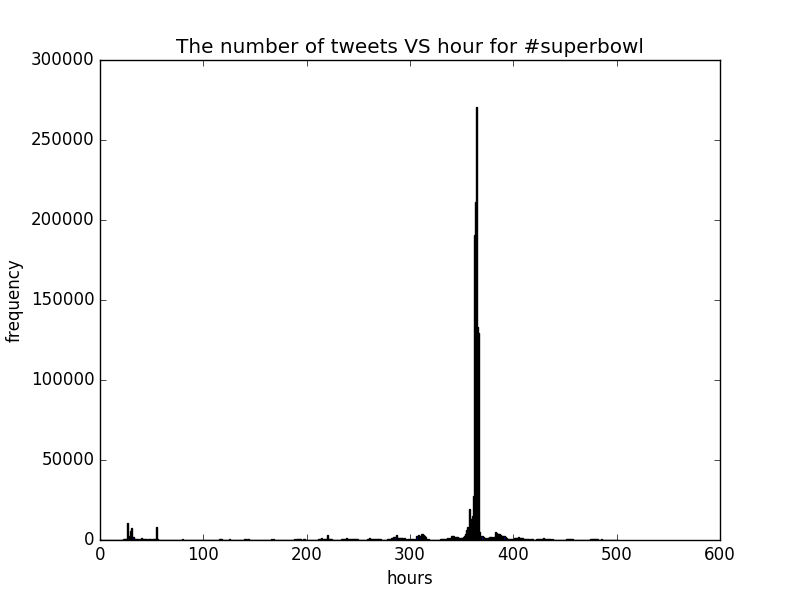
\includegraphics[width=.6\textwidth]{sp_hist.png}
\caption{The histogram for \#SuperBowl}
\label{fig:sp_hist}
\end{figure}
\begin{figure}[htbp]
\centering
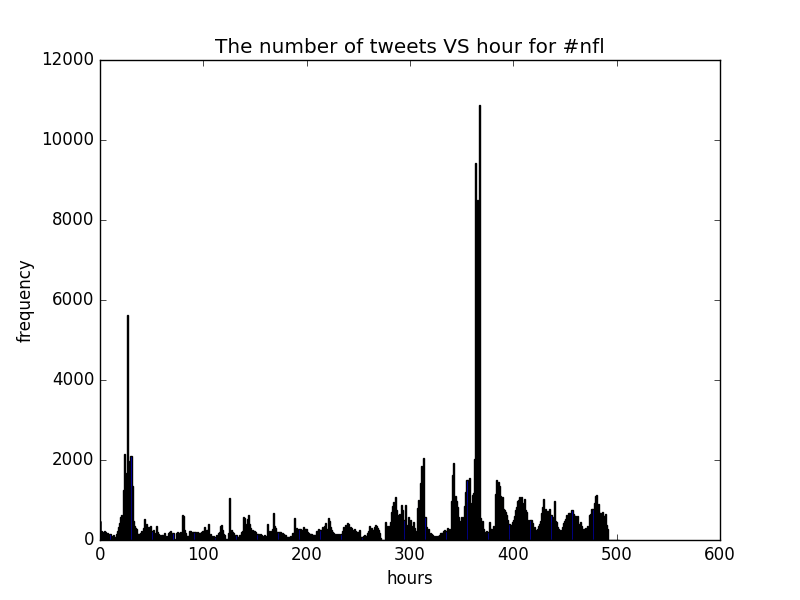
\includegraphics[width=.6\textwidth]{nfl_hist.png}
\caption{The histogram for \#NFL}
\label{fig:nfl_hist}
\end{figure}
\end{document}